\section{实验结果}

\subsection{性能收敛}

下图所示为训练过程示意图,从下图可以看出在进行16次迭代时,通过MEX性能函数已能看出在不断的训练中,
性能达到0.071.不难看出该网络模型的收敛速度较快。

\begin{figure}[ht]
	\centering
	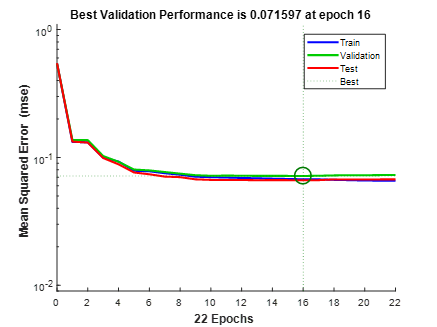
\includegraphics[width=.6\linewidth]{performance}
	\caption{神经网络训练结果}
	\label{fig:performance}
\end{figure}

\subsection{正确率87.5+\%}

\begin{table}[ht]
	\centering
	\caption{预测分布矩阵}
	\label{tab:eva}
	\begin{tabular}{cccc}
		& label 1 & label 2 & label 3 \\
		pred 1 & 95      & 32      & 1       \\
		pred 2 & 40      & 832     & 45      \\
		pred 3 & 1       & 28      & 109    
	\end{tabular}
\end{table}

我组通过多次训练,对网络参数进行修改,并且多次重新调整训练数据的维度和数量之后,
可以将训练模型的准确率基本稳定在86+\%,并且最佳模型高达87.57\%(如表~\ref{tab:eva})。